\documentclass[12p]{article}
\usepackage{latexsym}
\usepackage{lmodern}
\usepackage[T1]{fontenc}
\usepackage[spanish,activeacute]{babel}
\usepackage[utf8]{inputenc}
\usepackage{booktabs}
\usepackage{mathtools}
\usepackage{amssymb}
\usepackage{amsmath}
\usepackage{graphicx}
\usepackage{hyperref}
\usepackage{gensymb}
\usepackage{listings}
%\graphicspath{{Imagenes/}}
\usepackage[export]{adjustbox}[2011/08/13]

\setlength{\oddsidemargin}{-0.25in}
\setlength{\textwidth}{7in}
\setlength{\topmargin}{-.75in}
\setlength{\textheight}{9.2in}
\setlength{\parindent}{1cm}
\setlength{\parskip}{1ex}

\newcommand{\U}[1]{\,\mathrm{#1}}
\newcommand{\cels}{\U{{}^\circ}C}
\renewcommand{\baselinestretch}{1}\usepackage{lmodern}
\usepackage{listings} 
\usepackage{enumerate} 
\usepackage{rotating}


\title{Fenómenos de difracción en un láser diódico}
\author
{Gómez Arias, Andrés
\and
Navarrete Cruz, Erick Sebastián
\and 
Nellen Mondragón, Stefan Daniel
	}
\date{\today}

\begin{document}
\maketitle

\begin{abstract}
\noindent 
\end{abstract}

\section{Introducción}
\noindent La difracción es un fenómeno de ondas, que sucede generalmente cuando al propagarse la onda se encuentra con un obstáculo de geometría particular (de ``tamaño'' en el orden del $\lambda$). Para explicar esete fenómeno de forma clásica, se tiene que aplicar el principio de Huygens. Este principio dicta que en el frente de onda, todo punto se puede considerar como una fuente puntual de ondas. Introduciendo la amplitud compleja, U, una función de argumento complejo este principio se expresa cuantitativamente de la forma:
$$ U(\vec{x}) = -\frac{i}{\lambda} U(r_0) \int_{S} \frac {e^{iks}}{s} K(\chi)\,dS$$
Donde $k = \frac{2 \pi}{\lambda}$ y $r_0$ representa el radio de la onda primaria (fuente puntual), en un punto donde se forma un ángulo $\chi$ con la normal al circulo y la recta que una a dicho punto con $\vec{x}$. Por último, $K(\chi) = \frac{1}{2}(1 + \cos(\chi))$.
\par Ahora se consideran las aproximaciones debidas a Frauenhofer, que son validas para un campo lejano, es decir la distancia a una pantalla es mayor que el tamaño del obstáculo. Consideérese un obstáculo de ``tamaño'' $a$ y un observador a una distancia $L$ de la fuente de difracción. Sea $x \in \mathbb{R}$. La distancia de cualquier punto en el obstáculo al observador está dada por:
$$d = \sqrt{L^2 + (x + \frac{a}{2})^2}$$
si $$L >> (x + \frac{a}{2})$$ se obtiene la apoximación de Frauenhofer:
$$d \approx L + \frac{x^2}{2L}+\frac{x a}{2L}+\frac{a^2}{8L}$$
donde el último término se puede omitire si $\frac{a^2}{L} << \lambda$.
Dadas estas bases teóricas, se pueden empezar a resolver problemas concretos.
\par El primero de estos problemas es el de la difrección a través de una rendija simple. El principio de Bebinet indica que en el caso de una rendija simple y un obstáculo del mismo tamaño de la rendija, a largas deistancias, el patrón de interferencia es indsitinguible. Este es el caso para las aproximaciones empleadas, por lo que no se realiza un tratamienteo distinto para el cabello. Empleando las aproximaciones de Frauenhofer como limites para la integral de la amplitud compleja para la onda (que es un desarrollo bastante largo) $\Psi$, queda:
$$ \Psi = a \Psi^{\prime} \sqrt{\frac{i}{z\lambda}} \mathrm{sinc} \left( \frac{ka\sin\theta}{2} \right) $$
con $a$ el grosor de la rendija. Tomando el cuadrado de esto, para obtener la intensidad, queda:
$$I(\theta) = I_0 {\left( \operatorname{sinc} \left( \frac{\pi a}{\lambda} \sin \theta \right) \right) }^2$$
Donde $\sin(\theta) = \frac{x}{\sqrt{x^2 + L^2}}$. Así mismo, con la función de intensidad y notando la periodicidad de $\mathrm{sinc}$, se llega a que el growor del cabello, $w$ se encuentra en la expresión:
$$\frac{\pi W \Delta}{\lambda L} = 2\pi$$
siendo $\Delta x$ la distancia entre la primera y segunda franja.
\par Para un sistema de $n$ rendijas se considera la expresión
$$\Psi = \int_{D_i} \frac{i}{r\lambda} \Psi^\prime e^{-ikr}\,d\mathrm{D_i}$$
siendo D la rendija y $r$ la aproximación de Fresnel para dicha rendija. Por la linealidad de las ondasla contribución de cada una de ellas es aditiva. Queda:
$$\Psi = \sum_{i=0}^{n-1}\Psi_i$$
Después de integral y cuadrar $\Psi$ resulta que en el caso con $n = 2$
$$I(\theta) = \cos^2 \left ({\frac {\pi d \sin \theta}{\lambda}}\right)~\mathrm{sinc}^2 \left ( \frac {\pi a \sin \theta}{\lambda} \right)$$
con $a$ el grosor de las rendijas y $d$ la distancia entre estas.
\par Considérese ahora el caso del semiplano. Si $L$ es la distancia del observador al plano  y $x$ la posición lateral con respecto al haz,  se tiene la siguiente integrla para $U$:
$$U = \int_0^{\infty}\exp(ikL)\exp\left (ik\frac{(x-x')^2}{2L} \right ) \mathrm{d}x'$$
Esta integral no tiene solución cerrada. Sin embargo, debido a Sommerfeld, se puede expresar en términos de las funciones especiales (integrales de Fresnel) $S(x) = \int_0^x \sin(t^2)\,\mathrm{d}t$, $C(x) = \int_0^x \cos(t^2)\,\mathrm{d}t$ y $Fr(x) = C(x) + iS(X)$. Sommerfeld encontró (usando un método muy interesante, que se basa en interpretar una ``sábana'' de una superficie de asociada a la integral como el espacio físico) que la solución para $U$ es:
$U(\theta) = Fr\left(-2\sqrt{\frac{kr}{2}} \sin(\frac{\theta}{2}) \right) - Fr\left(-2\sqrt{\frac{kr}{2}} \cos(\frac{\theta}{2}) \right)$
donde $r = \sqrt{L^2 + x^2}$. Así $I = U^2$, que en efecto tiene imágen (y domino) real, pero su expresión no es más amigable.
\par Se espera poder observar los patrones descritos por las funciones de intensidad presentadas y ajustar los datos a estas funciones. Además, los datos relacionados, como el grosor del cabello, se esperan poder extraer de estos datos y ajustes.
 
\section{Materiales}

\section{Procedimiento}

\section{Datos experimentales}

Los datos experimentales correspondientes al patrón de difracción de un cabello y una rendija se muestran en la sección de resultados, incluidos con éstos.

Para la primera doble rendija se tomaron 3 imágenes con diferentes brillos y contrastes (para que en algunas se apreciara la franja central y en otras las laterales). Para la segunda doble rendija se tomaron 2. Para el semiplano se tomaron 2, pero se tomó en cuenta la de menos brillo (menos saturación).

\begin{figure}[h]
  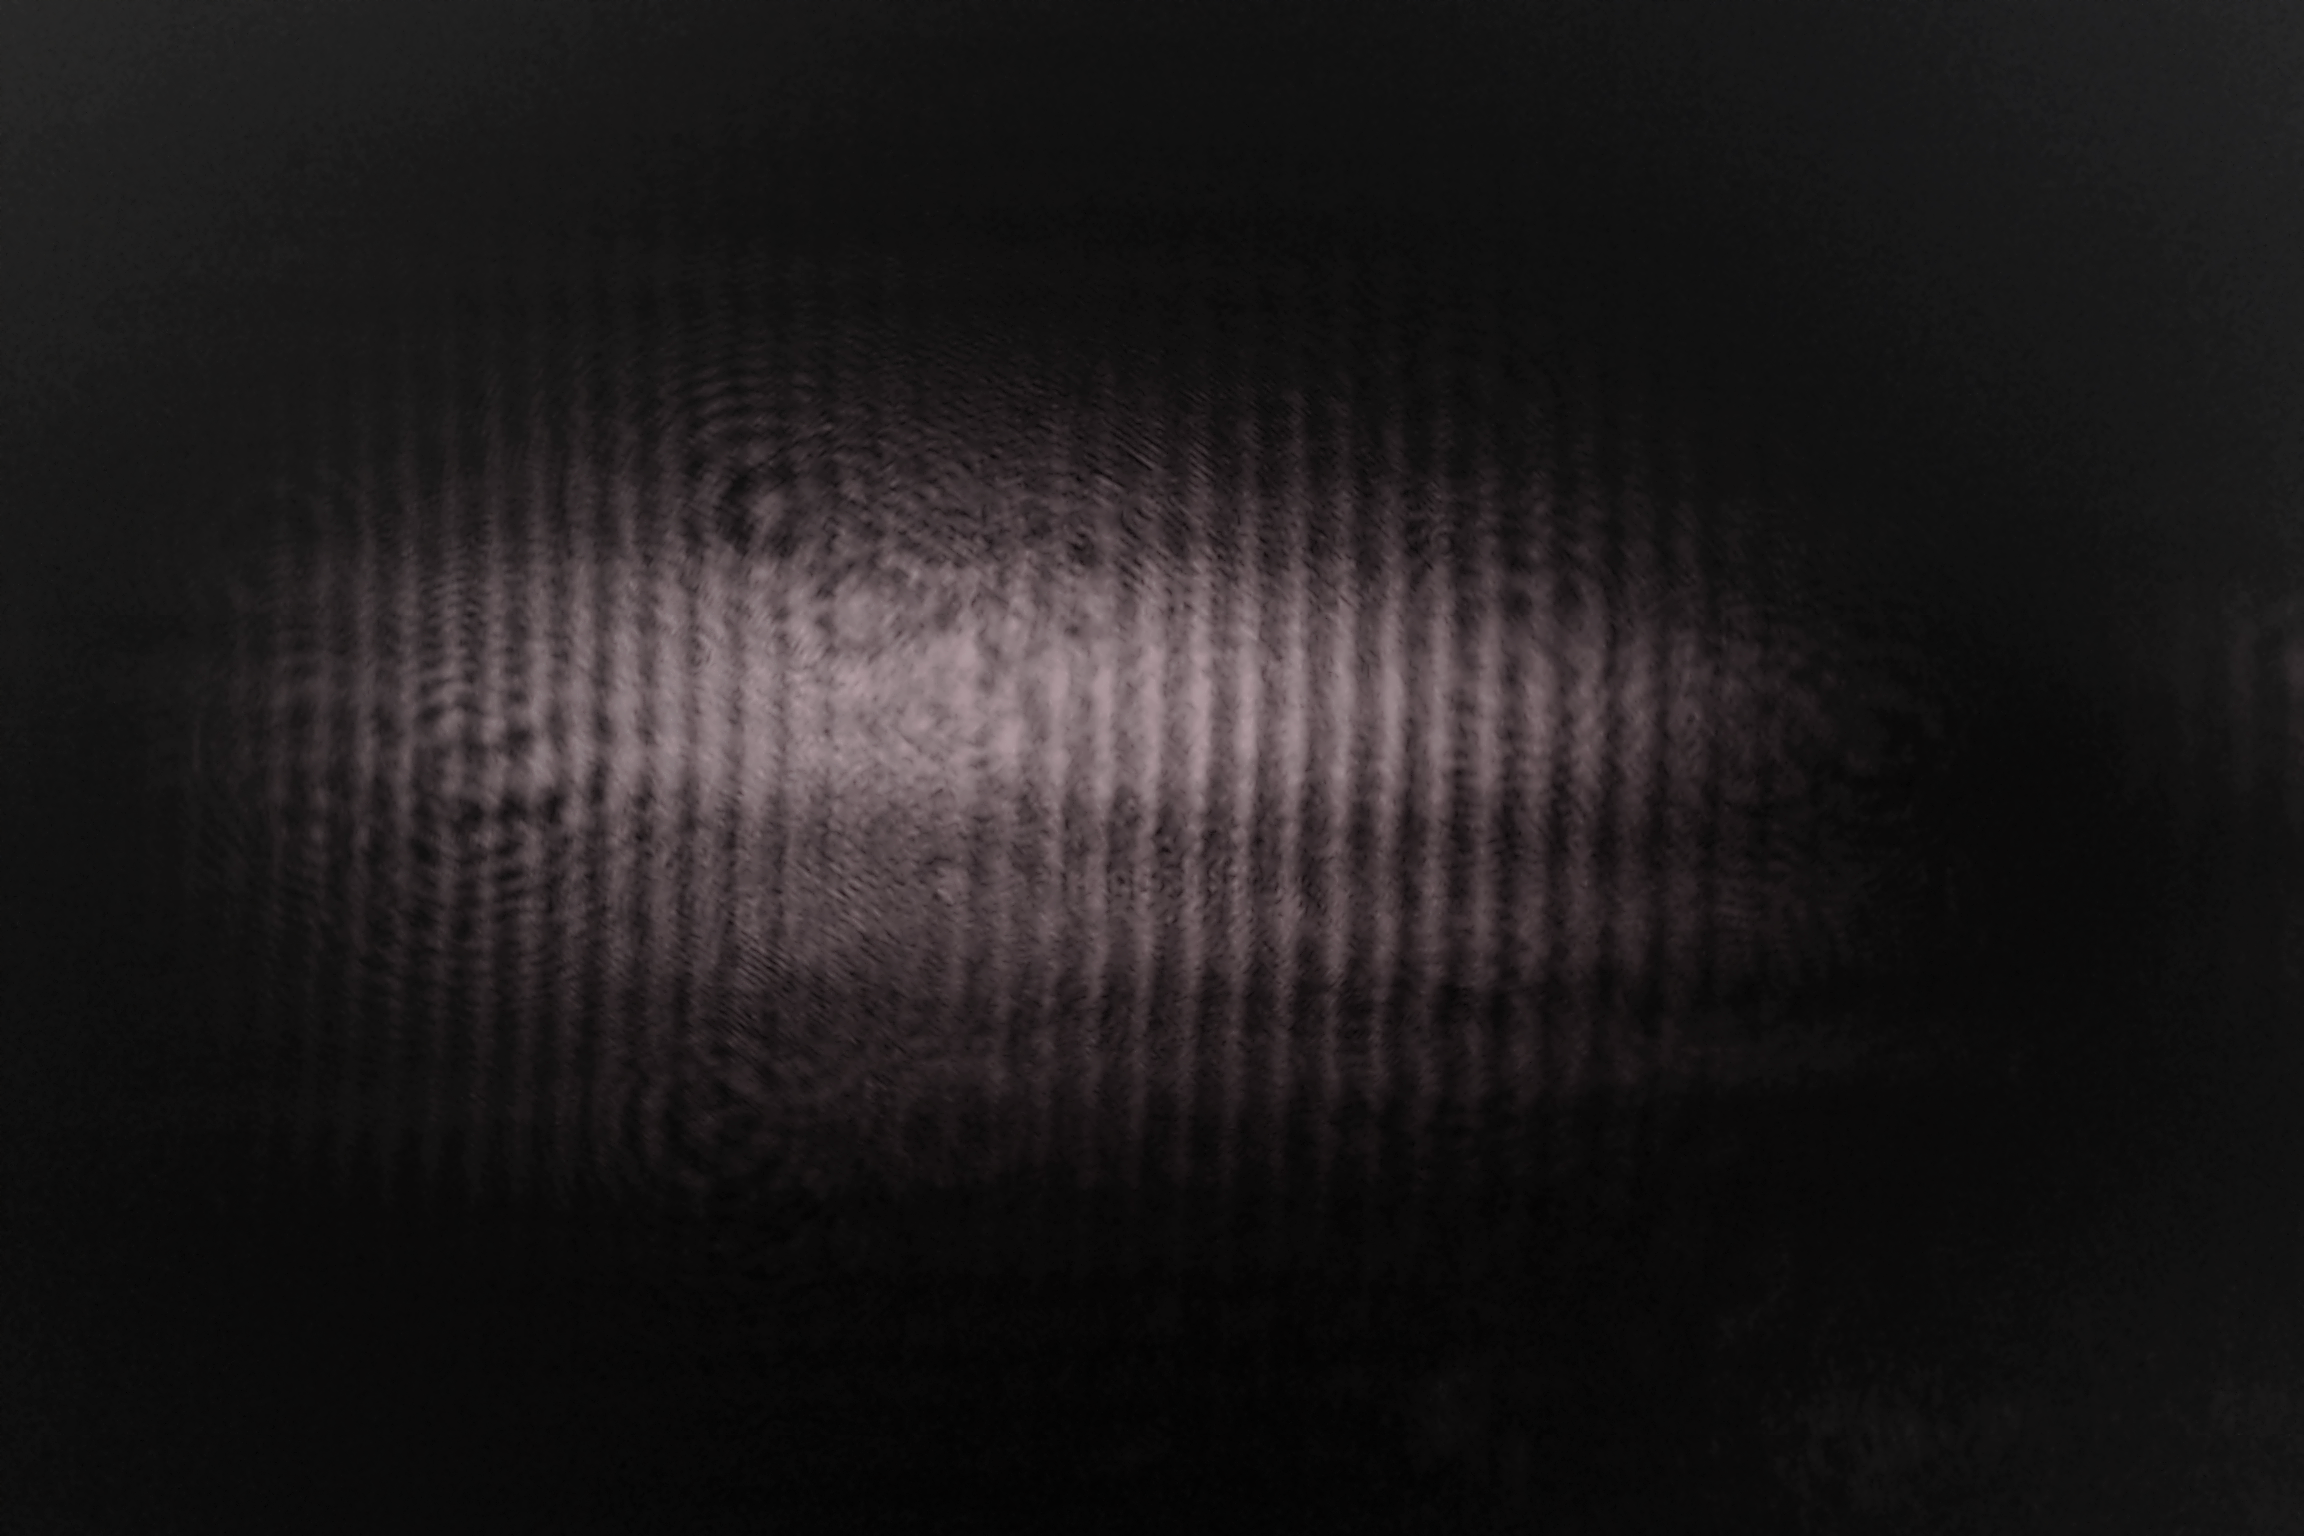
\includegraphics[width=0.6\textwidth]{1.png}
  \centering
  \caption{Rendija 1, imagen 1}
\end{figure} 

\begin{figure}[h]
  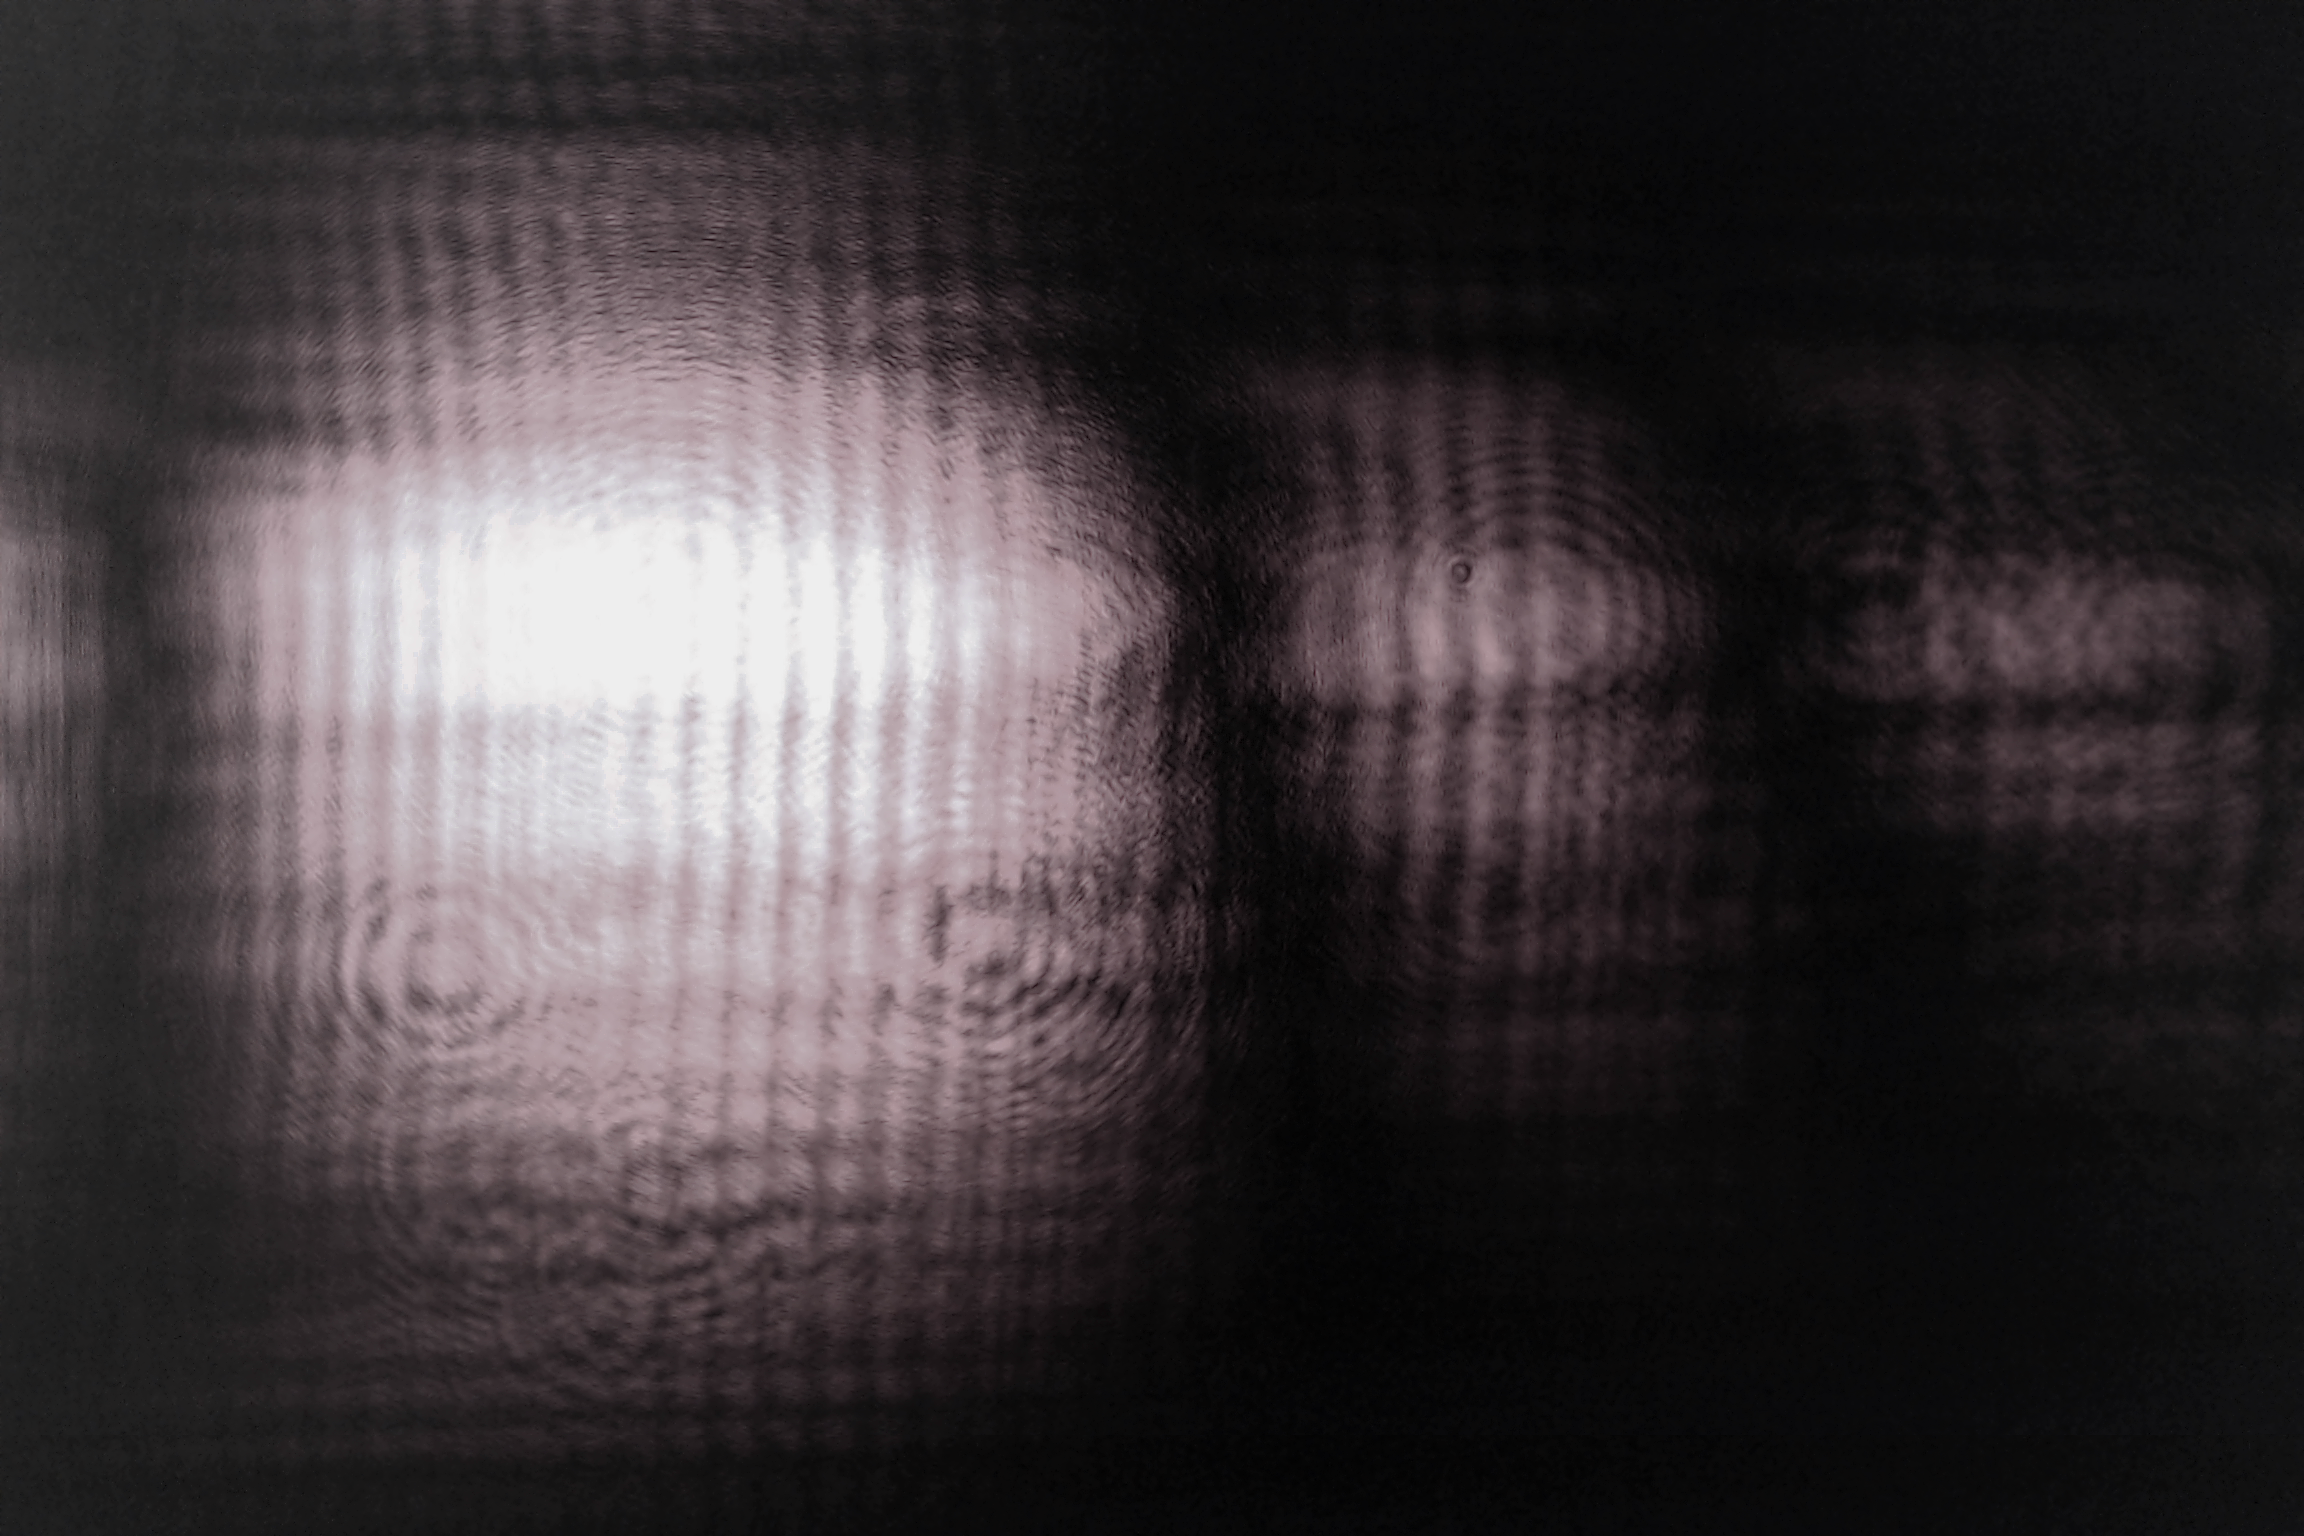
\includegraphics[width=0.6\textwidth]{2.png}
  \centering
  \caption{Rendija 1, imagen 2}
\end{figure} 

\begin{figure}[h]
  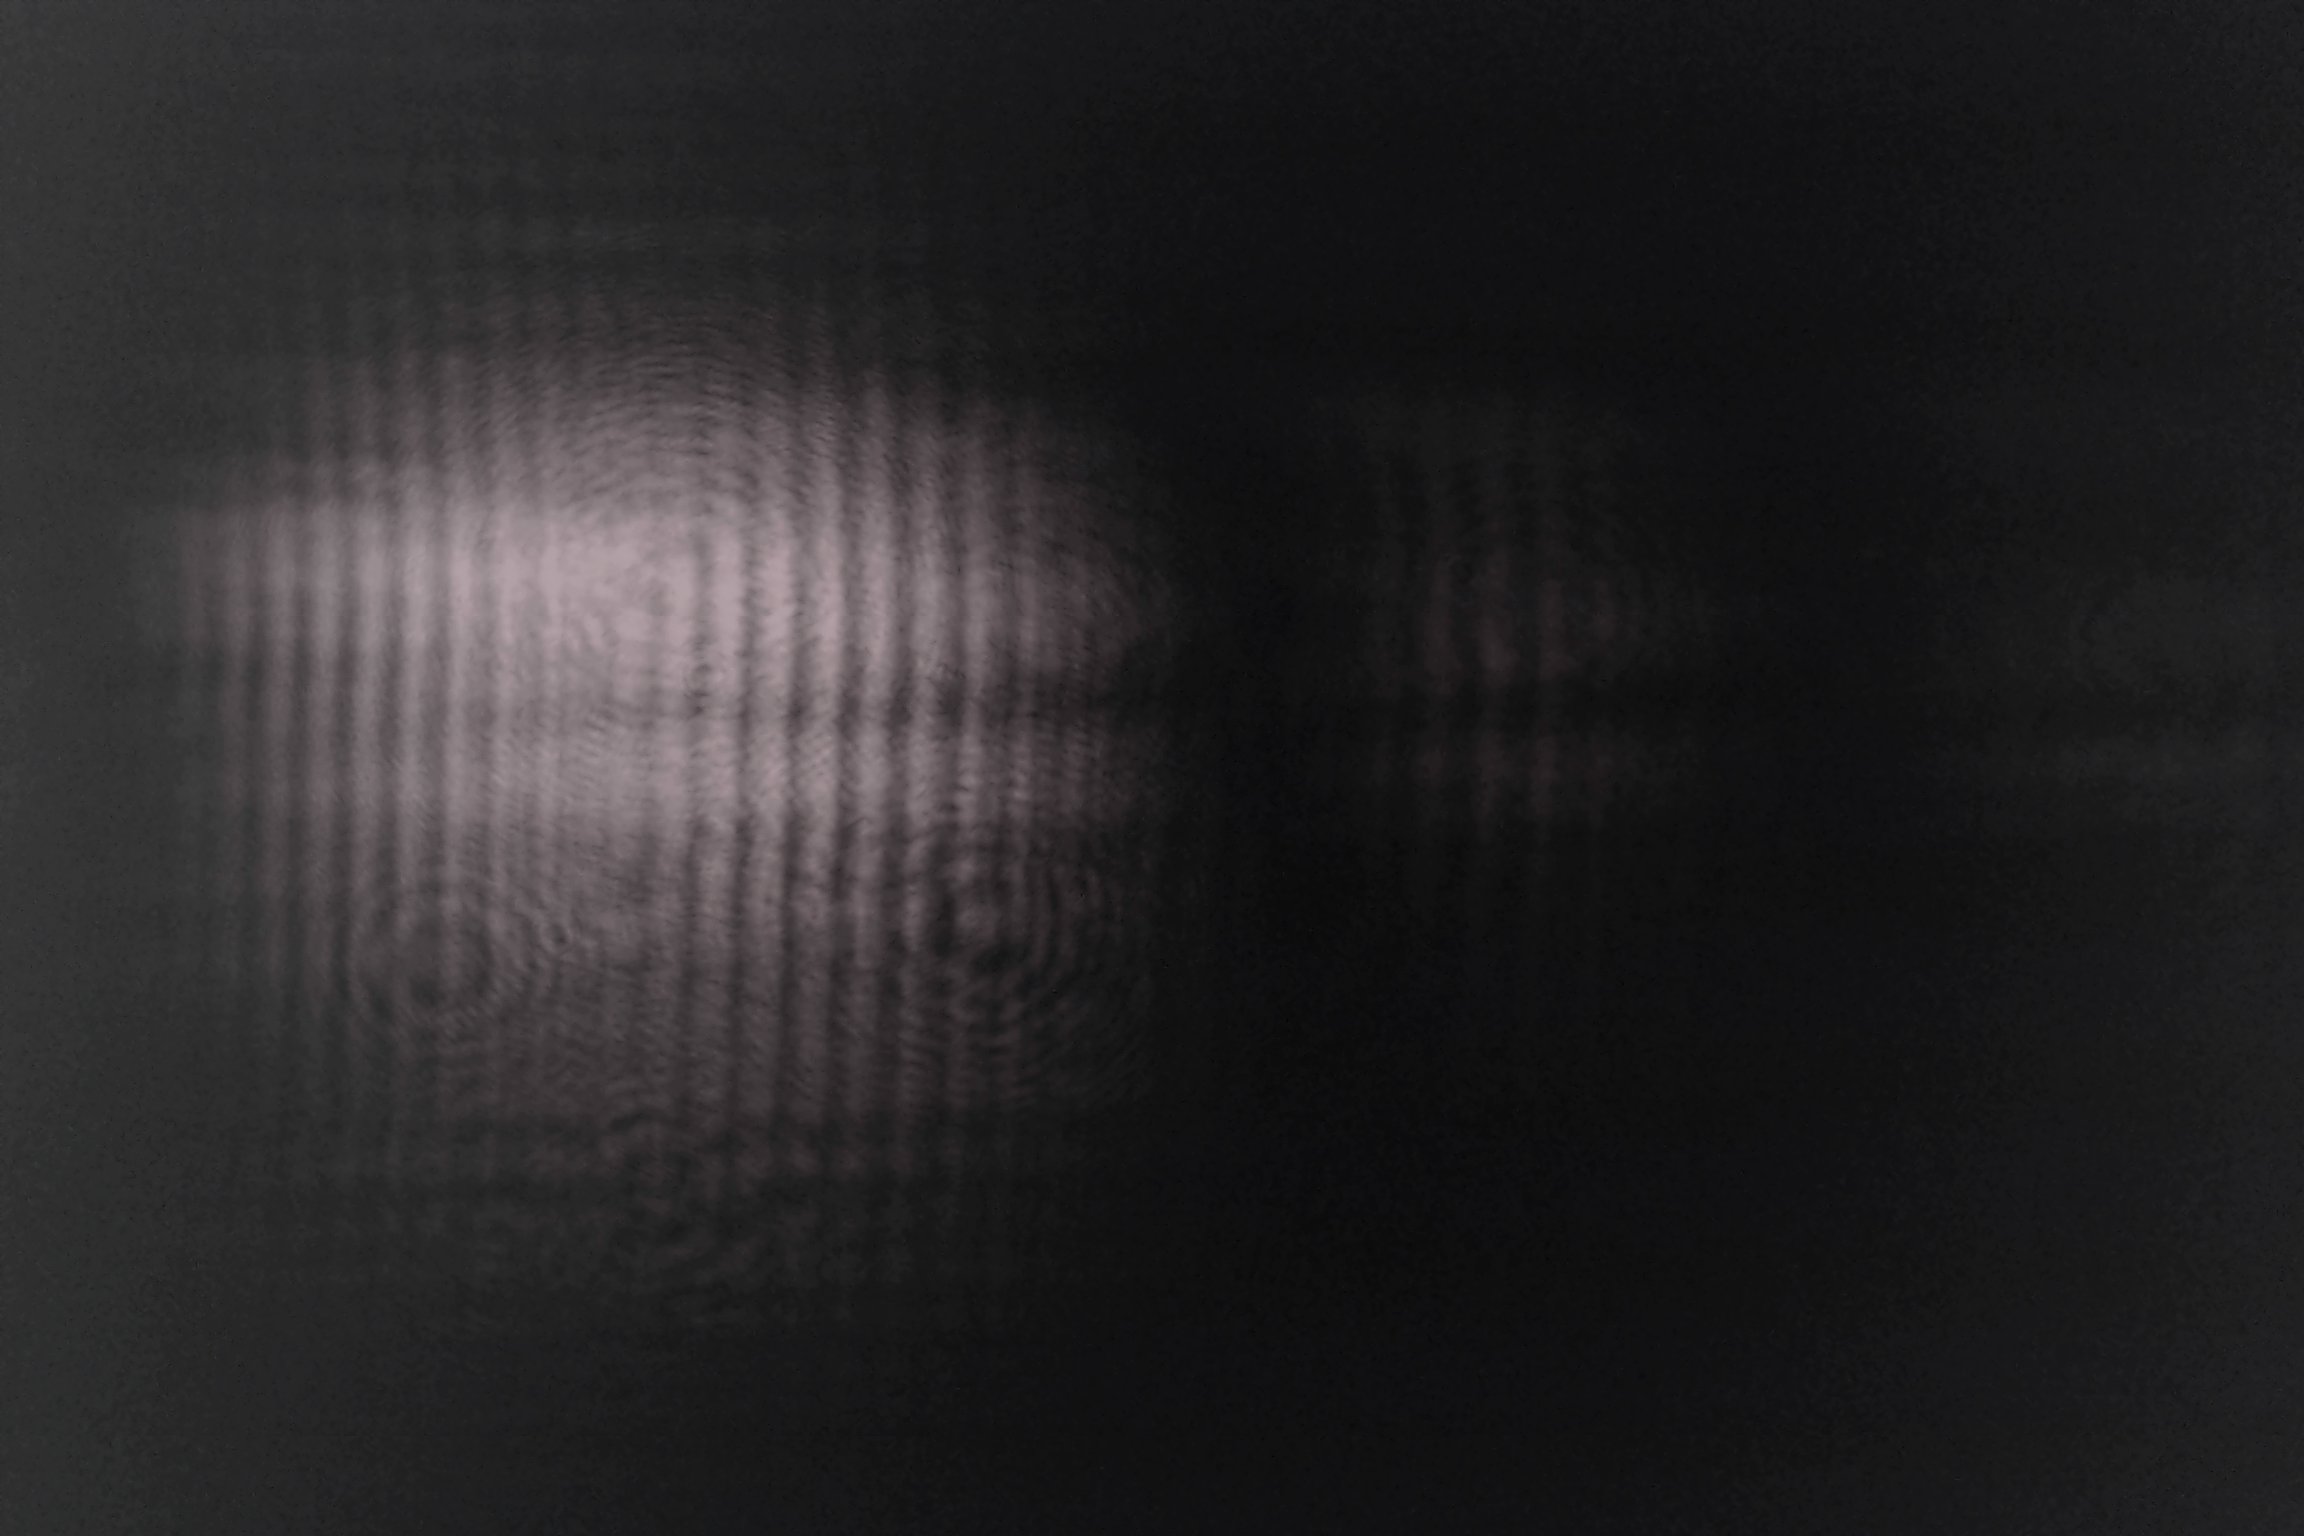
\includegraphics[width=0.6\textwidth]{3.png}
  \centering
  \caption{Rendija 1, imagen 3}
\end{figure} 

\begin{figure}[h]
  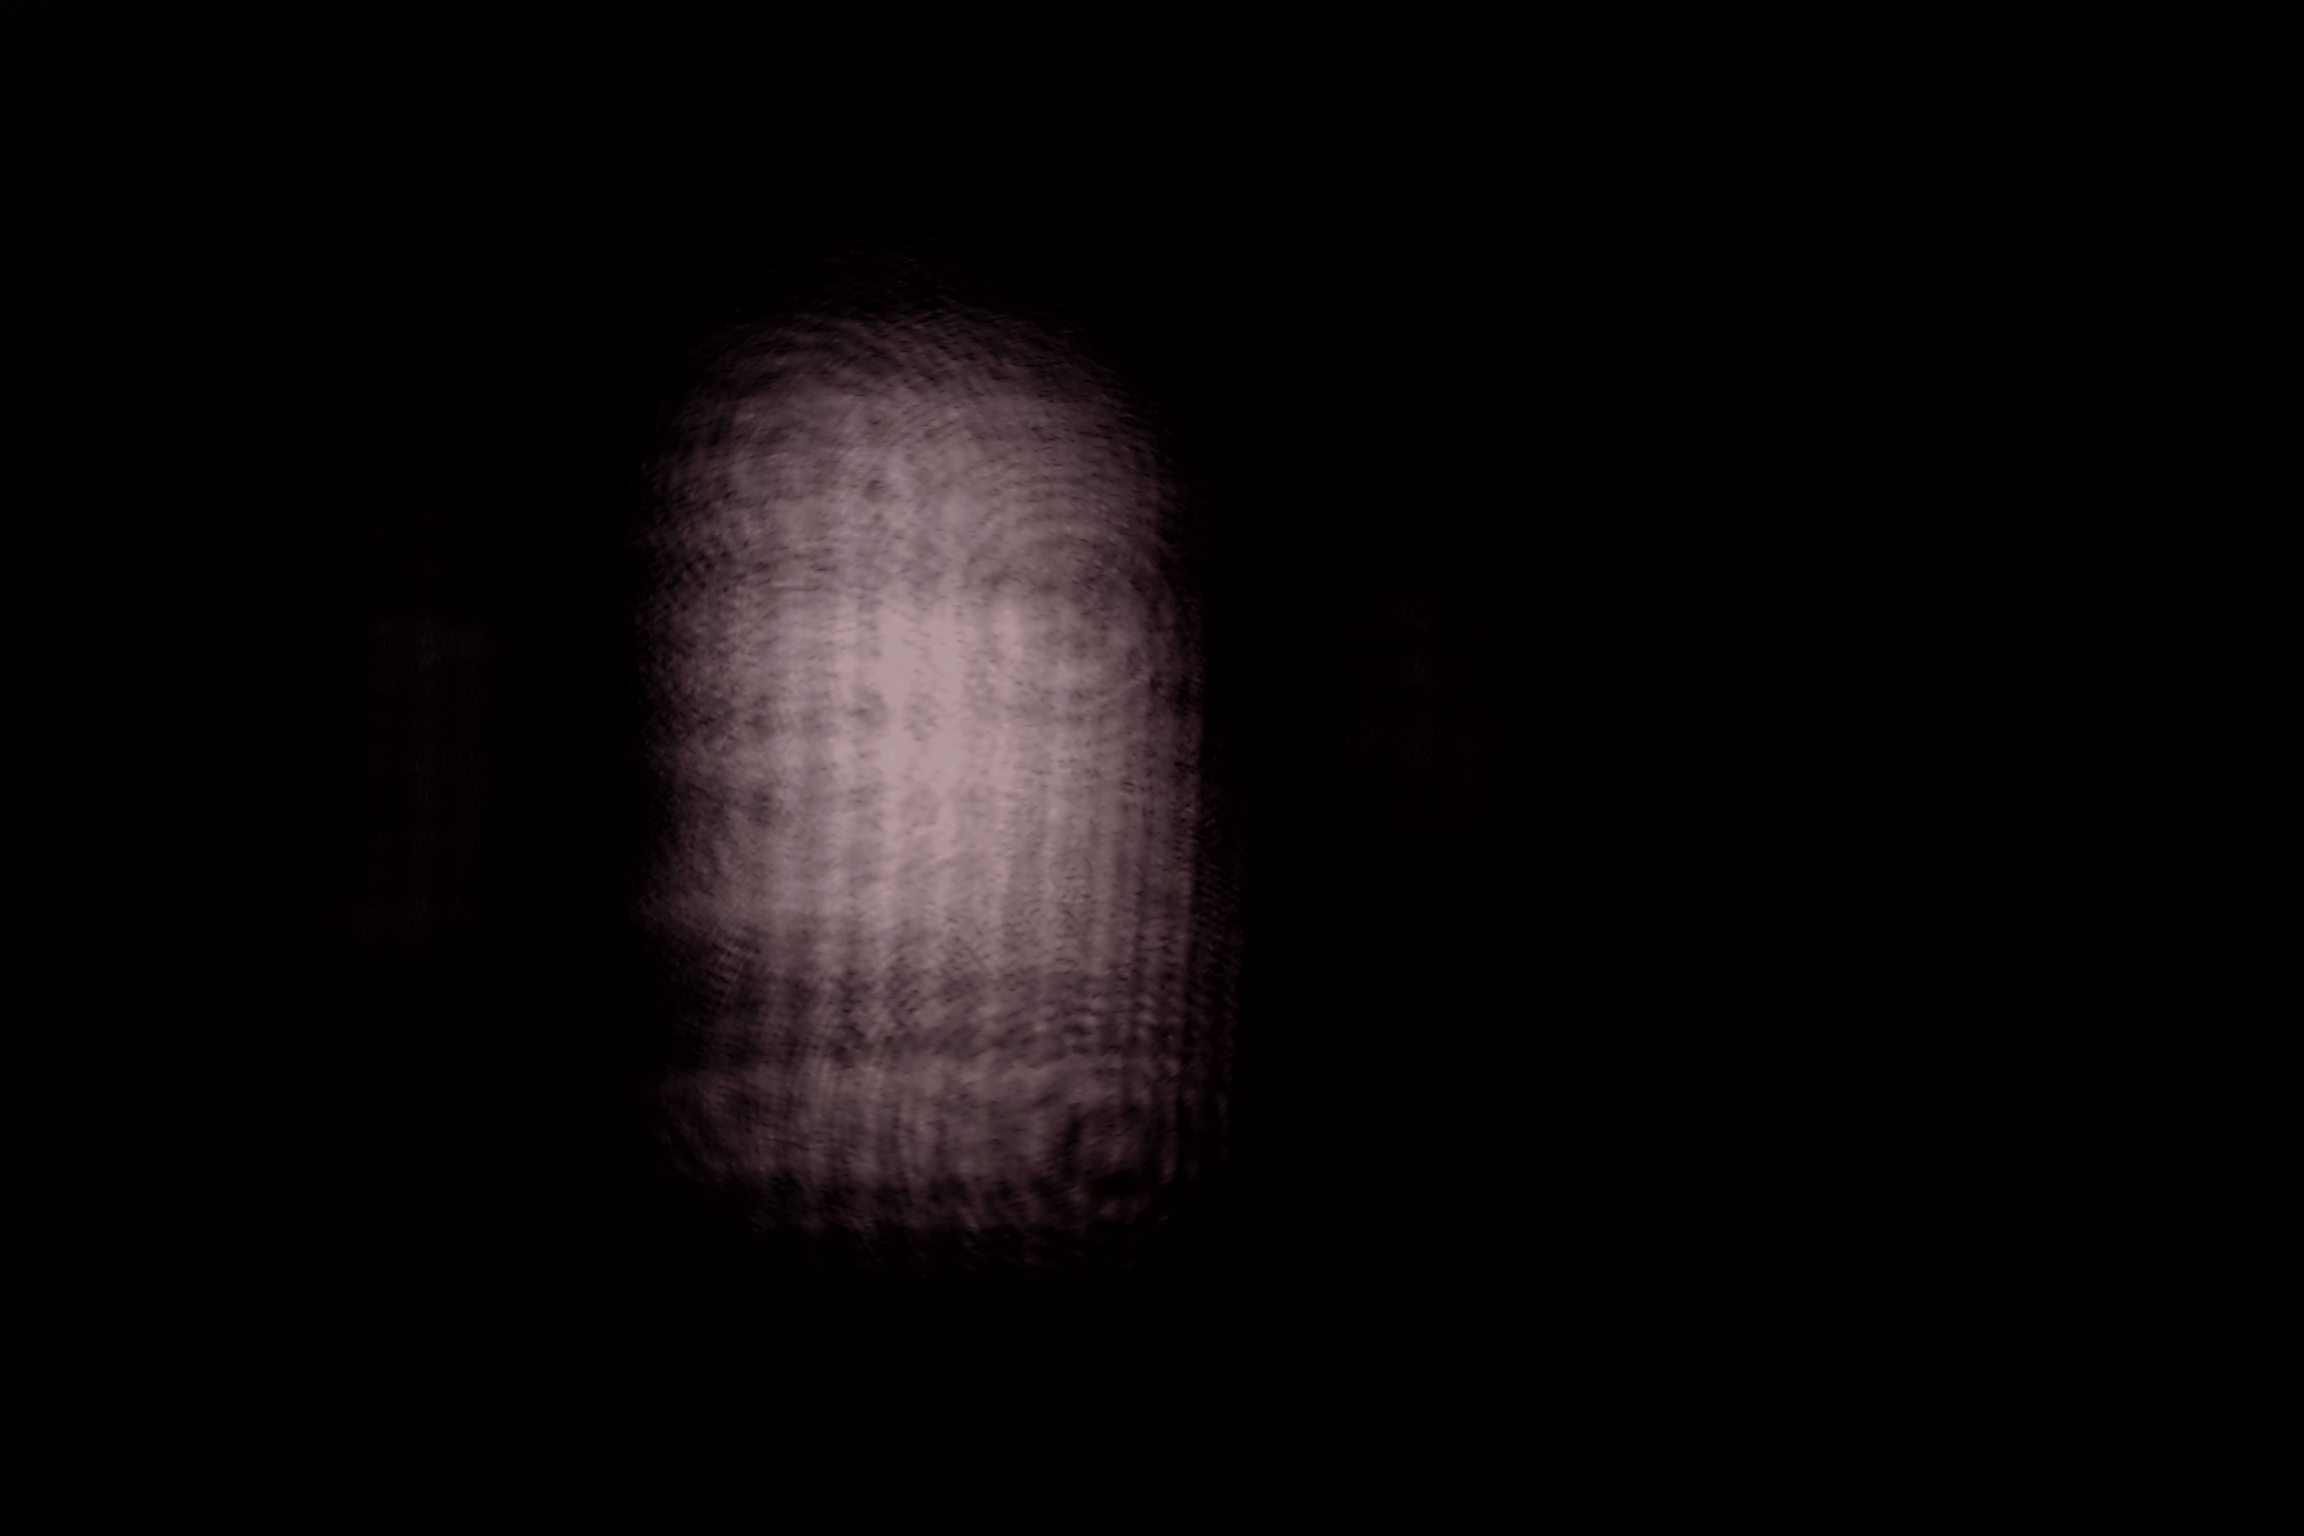
\includegraphics[width=0.6\textwidth]{a.png}
  \centering
  \caption{Rendija 2, imagen 1}
\end{figure} 

\begin{figure}[h]
  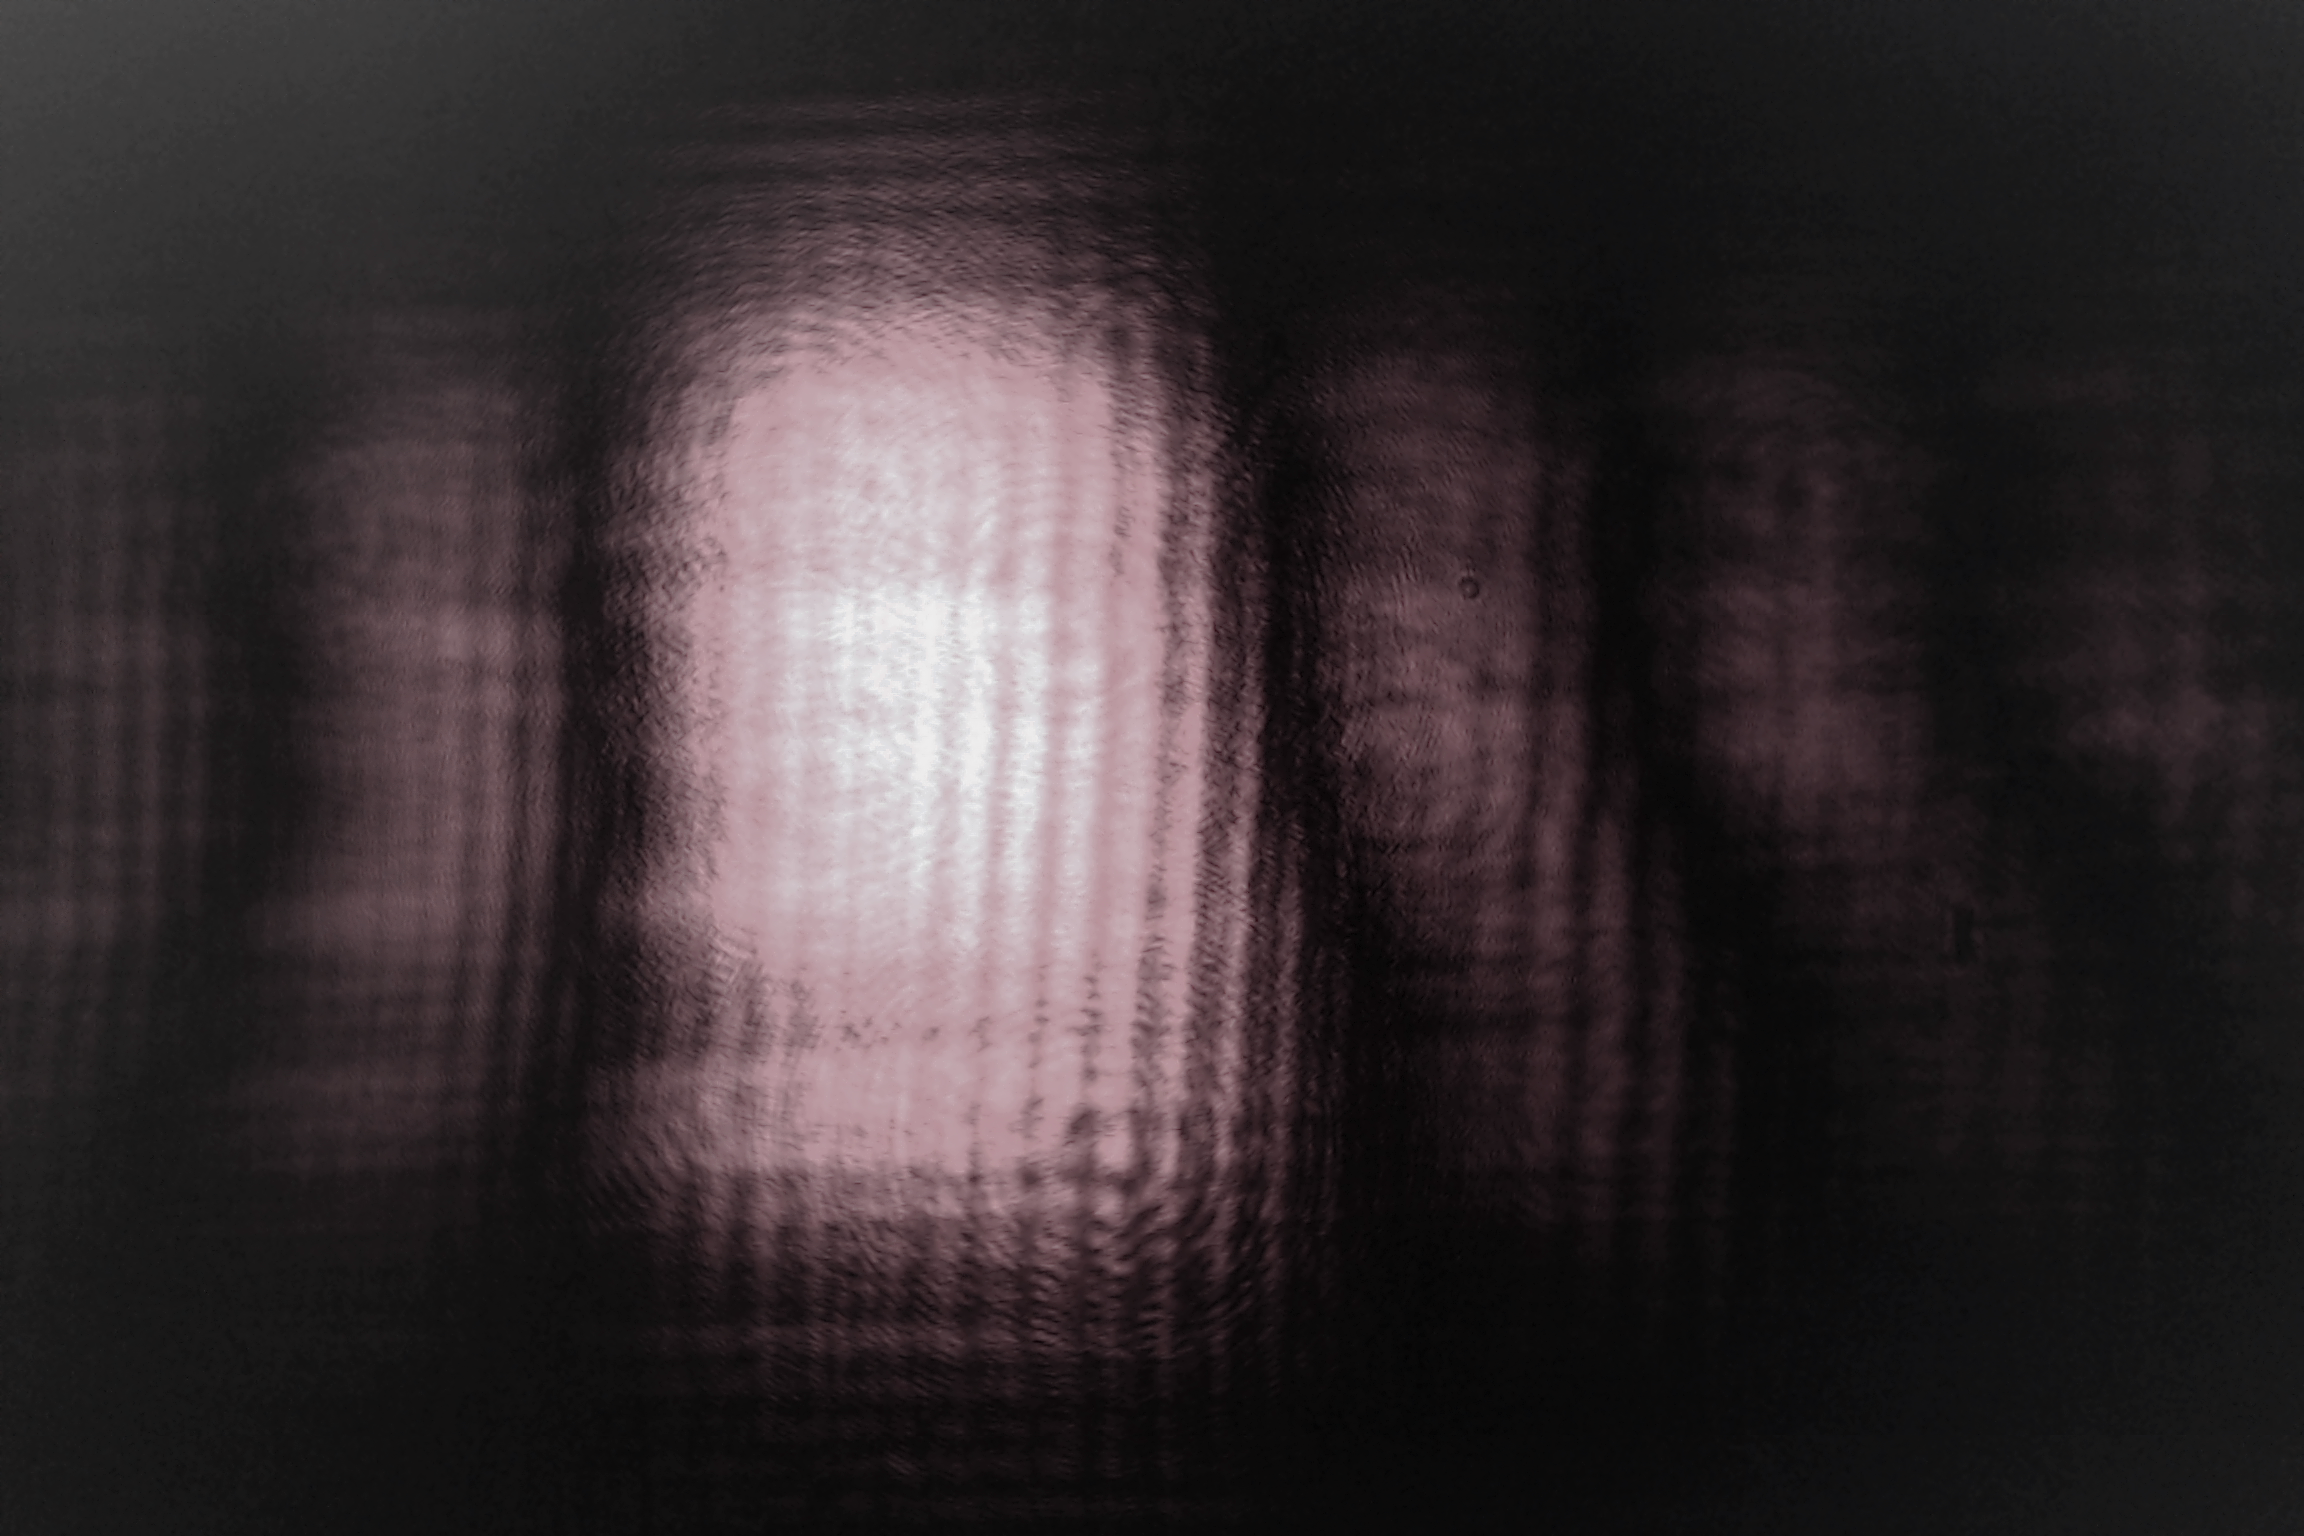
\includegraphics[width=0.6\textwidth]{b.png}
  \centering
  \caption{Rendija 2, imagen 2}
\end{figure} 

\begin{figure}[h]
  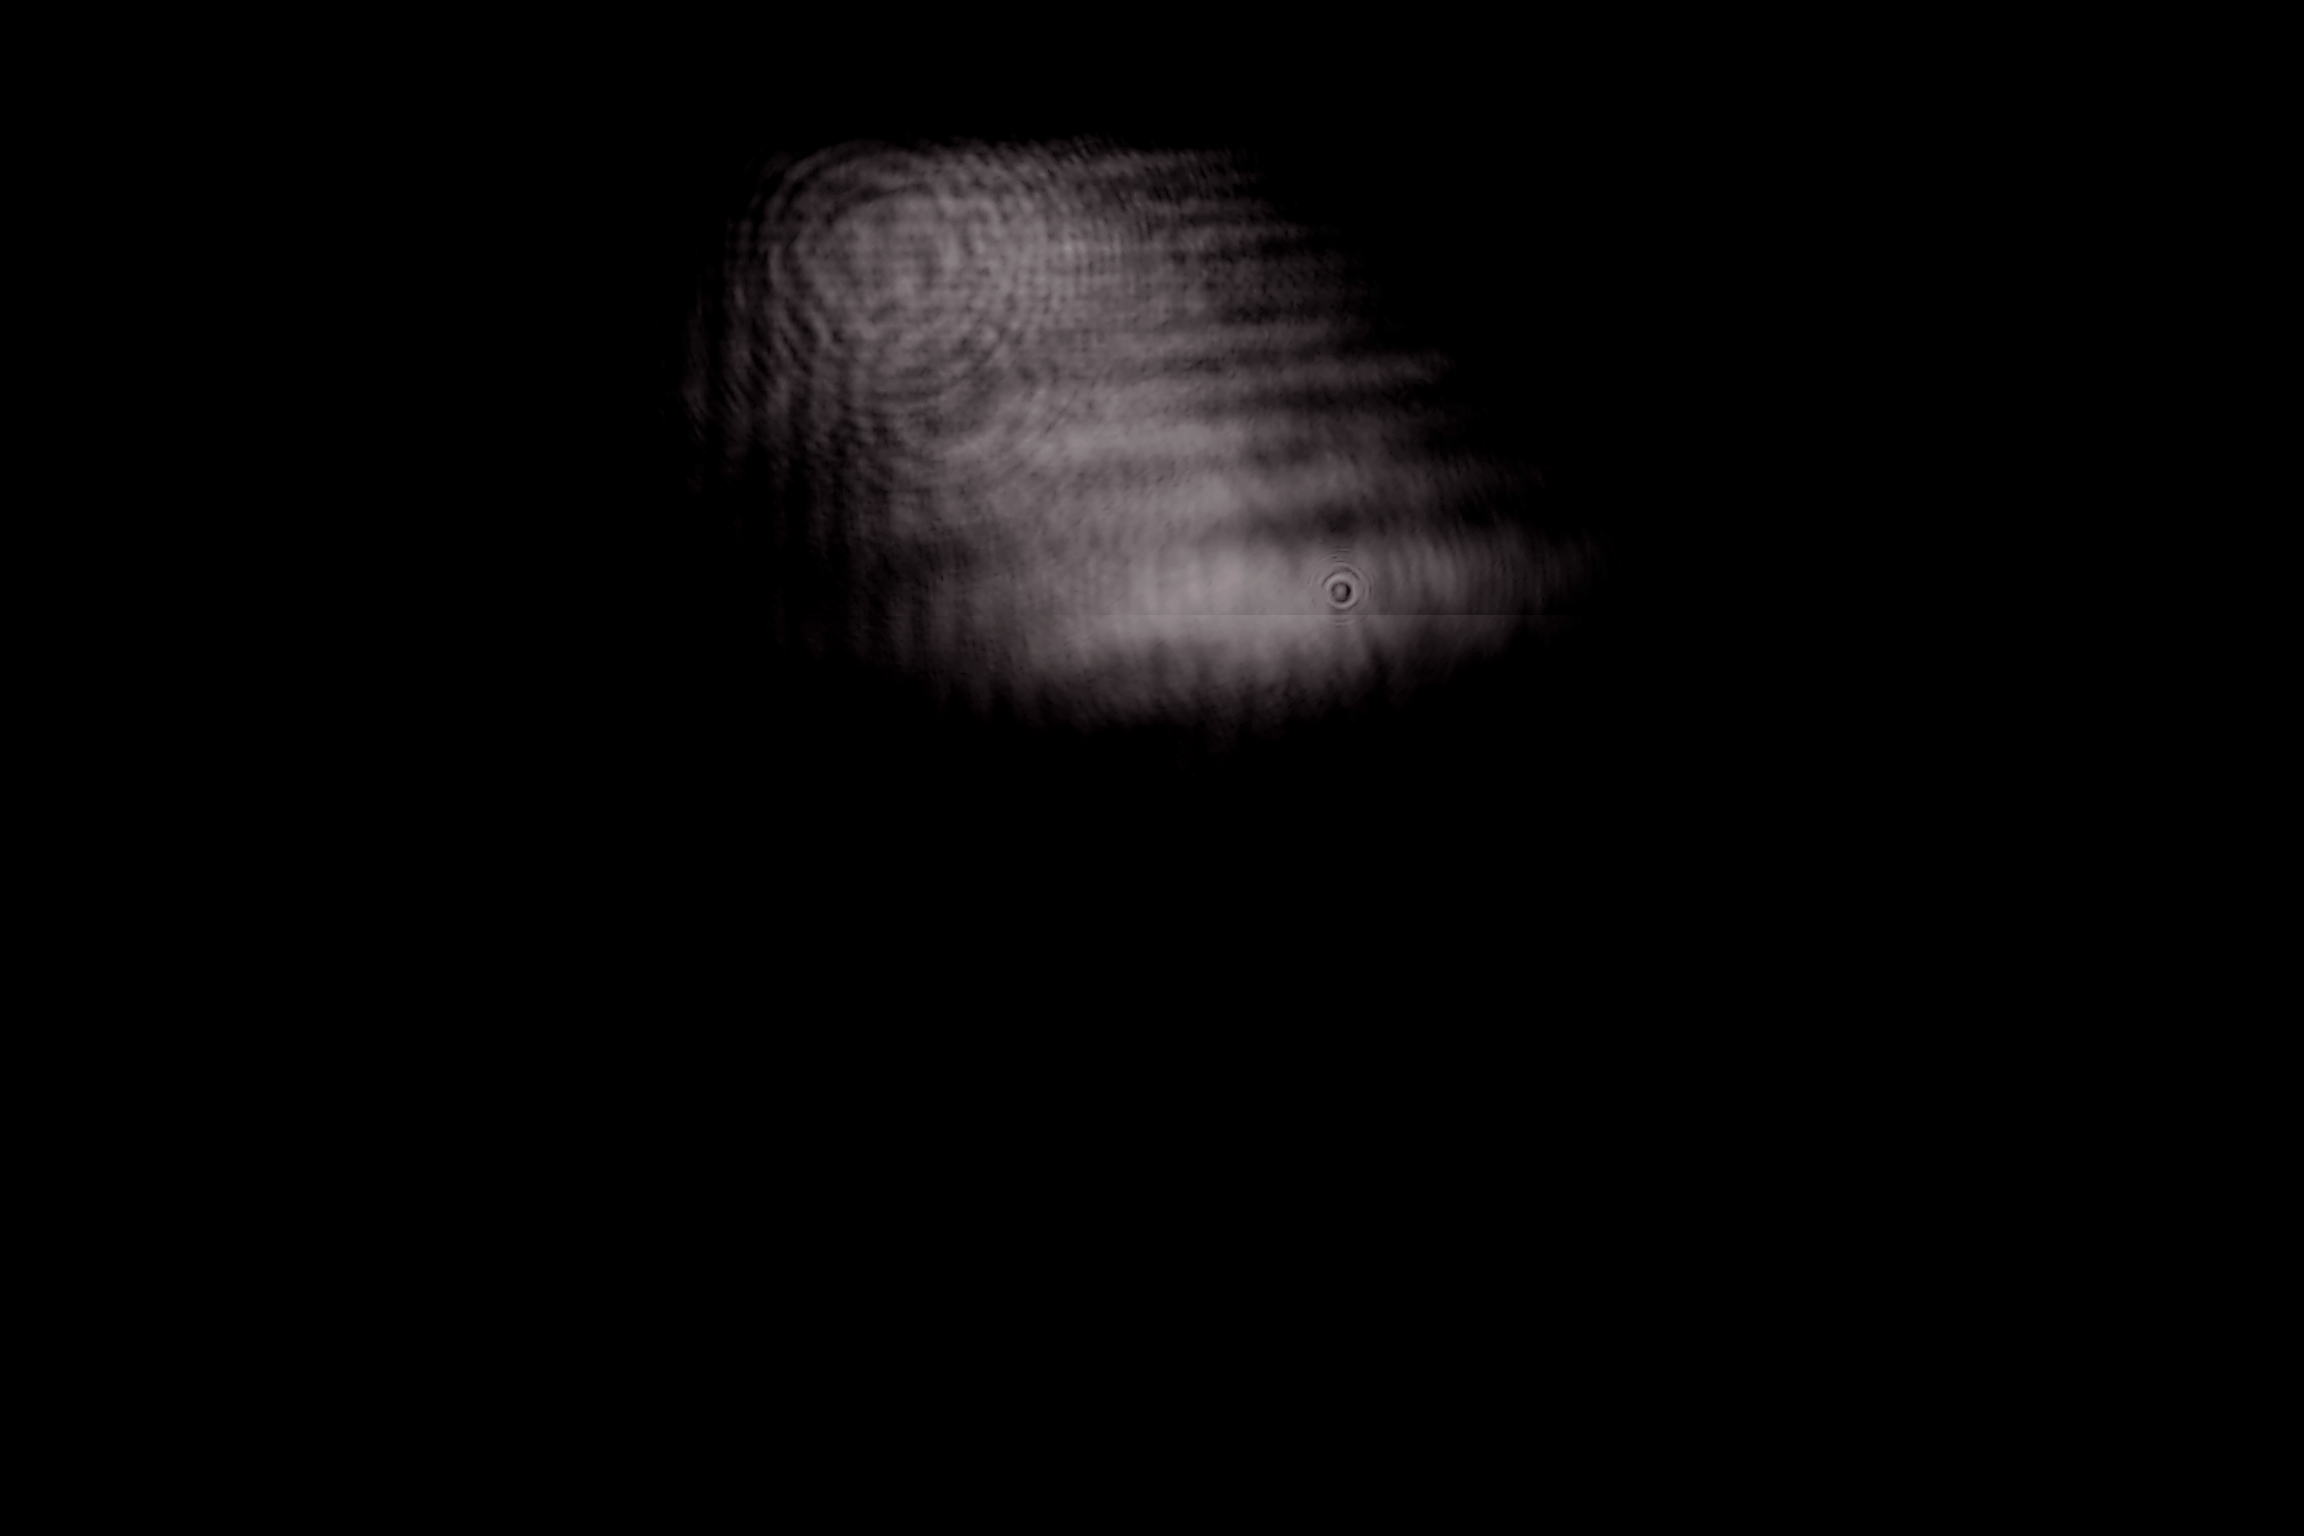
\includegraphics[width=0.6\textwidth]{sp.png}
  \centering
  \caption{Semiplano (barrera en la parte inferior del patrón)}
\end{figure} 

\section{Resultados}

A continuación se muestran los resultados referentes al patrón de interferencia del cabello y la rendija simple. Donde $z$ es la distancia del cabello o rendija a la pantalla en donde se proyectaba el patrón, $\Delta x$ es la anchura de la franja principal y consecuentemente $Wx$ es el diámetro del cabello o anchura de la rendija, respectivamente (obtenido directamente de la fórumla). El error inusual de $z$ en el segundo experimento de la rendija simple se debe a que por accidente se movió la rendija un poco antes de medir $z$.

Cabello:

\begin{tabular}{lllllll}
\toprule
{} & z[mm] & dz[mm] & $\Delta x$[mm] & $d\Delta x$[mm] & Wx[$\mu m$] & dWx[$\mu m$] \\
\midrule
0 &  2622 &    0.5 &      41 &       1 &   81 &    2 \\
1 &  2015 &    0.5 &      51 &       1 &   50 &    1 \\
2 &   972 &    0.5 &      20 &       1 &   60 &    3 \\
\bottomrule
\end{tabular}

Rendija simple:

\begin{tabular}{lllllll}
\toprule
{} & z[mm] & dz[mm] & $\Delta x$[mm] & $d\Delta x$[mm] & Wx[$\mu m$] & dWx[$\mu m$] \\
\midrule
0 &  2549 &    0.5 &      53 &       1 &   61 &    1 \\
1 &  2017 &     20 &      39 &       1 &   66 &    2 \\
2 &  1085 &    0.5 &    22 &       1 &   63 &    3 \\
\bottomrule
\end{tabular}

En los patrones de interferencia de las dobles rendijas, debido a que en la primera imagen no se podían observar las franjas laterales en el patrón de interferencia, aunado con que ésta es la de peor calidad de las tres, ésta no se tomó en cuenta. Para el resto de las imágenes se hizo un corte de una hilera horizontal (vertical para el semiplano) con altura dada por 1 pixel. De manera que podamos graficar en 1 dimensión la intensidad de luz con respecto a x (con respecto a y en el semiplano). Ésto se hizo en el editor de imágenes paint, usando las hileras (columna) centrales que menos ruido tenían y que mejor aspecto daban del patrón de interferencia. Las imágenes con dichas hileras se incluyen en el anexo de éste reporte, junto con algunas gráficas en 2D de los patrones de interferencia. Para trabjar con las hileras de pixeles se utilizó la paquetería scipy y numpy de python para análisis de imágenes y análisis estadístico. Éstas se transformaron a escala de grises y se normalizaron. De modo que el 0 es la menor intensidad y 1 es la mayor intensidad (intensidad de 256 en la escala de grises).

Se tuvieron que hacer varios retoques a las gráficas y ajustes: Para centrar en el máximo se hizo un promedio pesado de la posición de los 10 puntos con mayor intensidad, con la función peso variando linealmente de 1 hasta 10 (peso 1 para el decimo mayor y peso 10 para el mayor). Ésto debido a que cualquier ruido en la cresta de la franja principal causaba que hubiera un máximo global ligeramente al lado del "centro de masa" de la distribución, lo que afectaba seriamente al ajuste. Hecho esto se ponía el origen en dicha ubicación. Análogamente, de manera ideal el cero de la intensidad de luz hubiera sido el mínimo de intensidad de toda la distribución. Pero de nuevo se tenían picos provocados por ruido que causaban una traslación vertical de todo el conjunto de datos, afectando seriamente el ajuste. Ésto se arregló a mano; trasladando todo el conjunto de datos de manera que el mínimo geométrico (el punto donde la derivada se hacía cero) tocara tangencialmente al eje de intensidad cero.

Por último, se encontraron las dimensiones del sensor con otro modelo de cámara (Logitech C920 HD PRO) que tiene el mismo sensor. Éste mide 5.14mm por 3.50mm. Las imágenes eran de 2304px por 1536px. Dejando el ancho de cada pixel en $2.23\mu m$ y altura en $2.28\mu m$.

A continuación se muestran las gráficas de la intensidad (azul), primero ajustadas al término de $sinc^2$ (la envolvente, en rojo) y luego con los parametros obtenidos, ajustadas al modelo completo, que incluye el término $cos^2$ (turquesa). En la discusión se hablará de porqué en algunas gráficas no hay ajuste.

Para rendija 1, imagen 3 se obtuvo que $a=45 \mu m$ y $b=1657 \mu m$.

Para rendija 2, imagen 1 se obtuvo que $a=80 \mu m$ y $b=2300 \mu m$

\begin{figure}[h]
  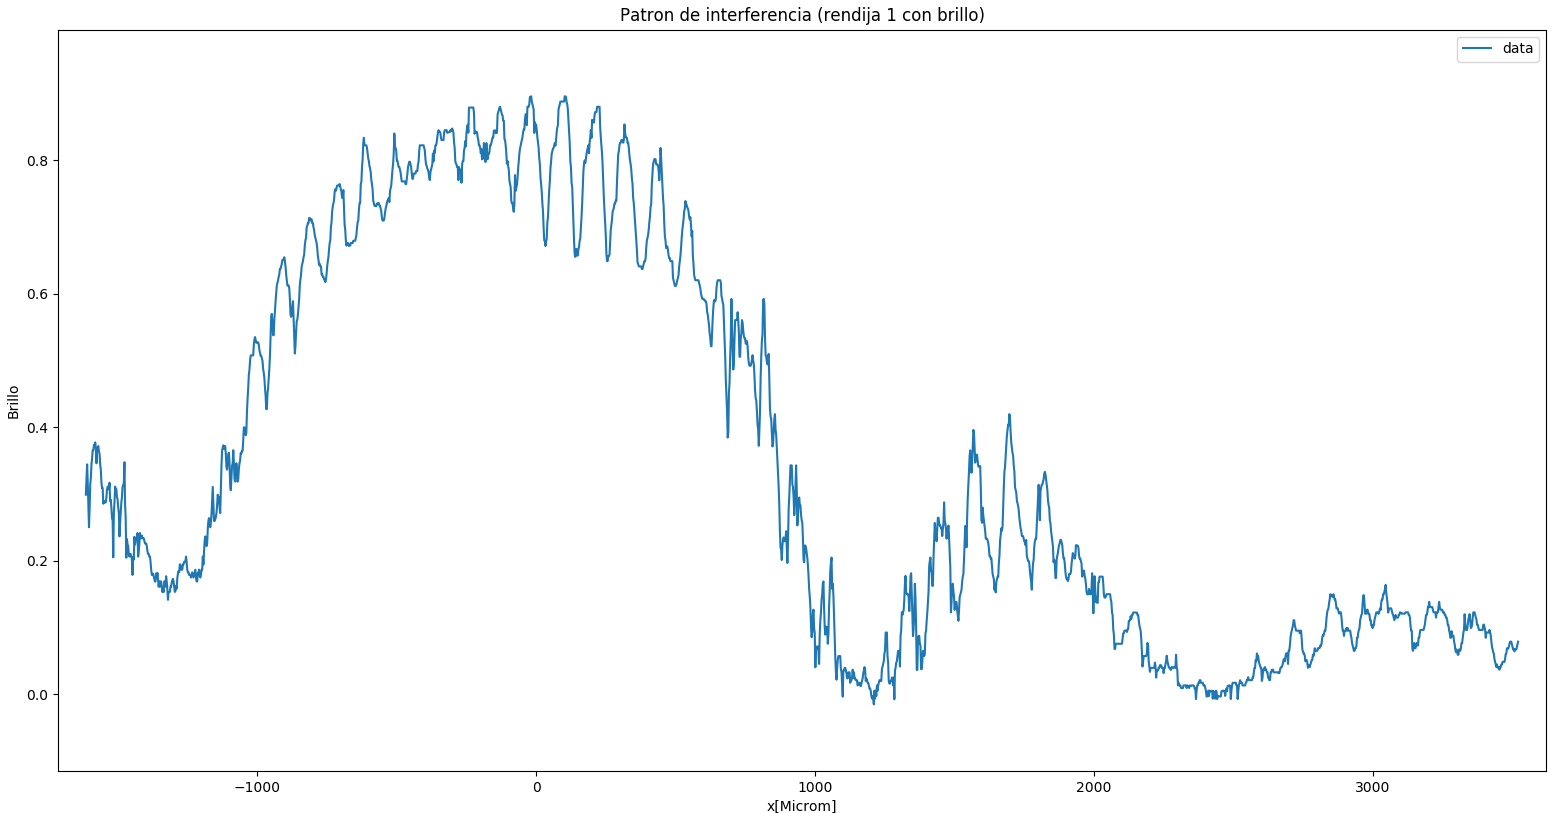
\includegraphics[width=1.0\textwidth]{2pg.png}
  \centering
  \caption{Gráfica en del brillo de una hilera de la imagen de doble rendija (Rendija 1, imagen 2)}
\end{figure}

\begin{figure}[h]
  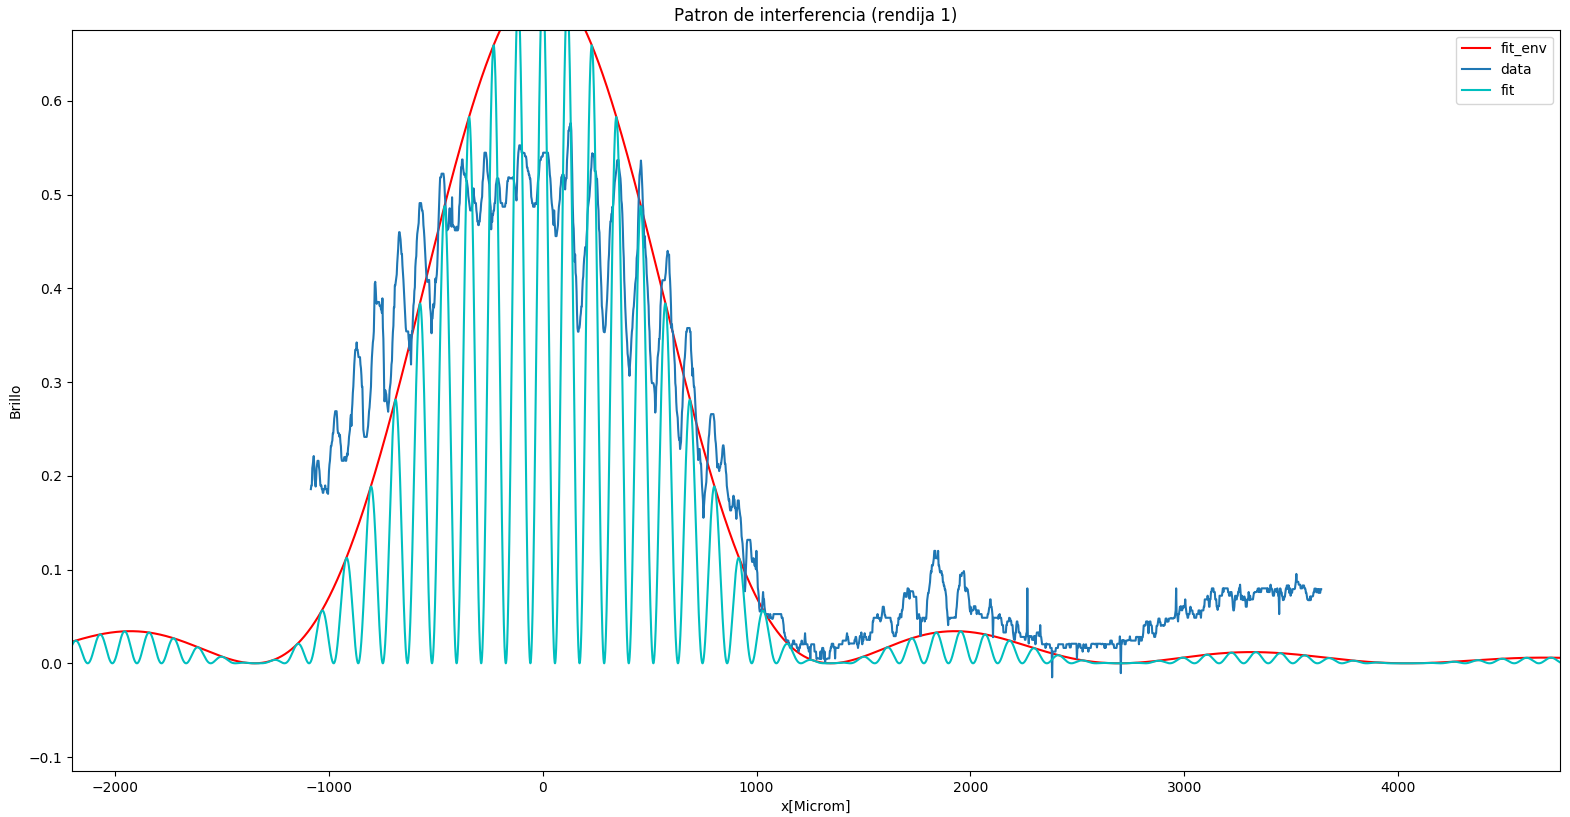
\includegraphics[width=1.0\textwidth]{3pg.png}
  \centering
  \caption{Gráfica en del brillo de una hilera de la imagen de doble rendija (Rendija 1, imagen 3)}
\end{figure} 

\begin{figure}[h]
  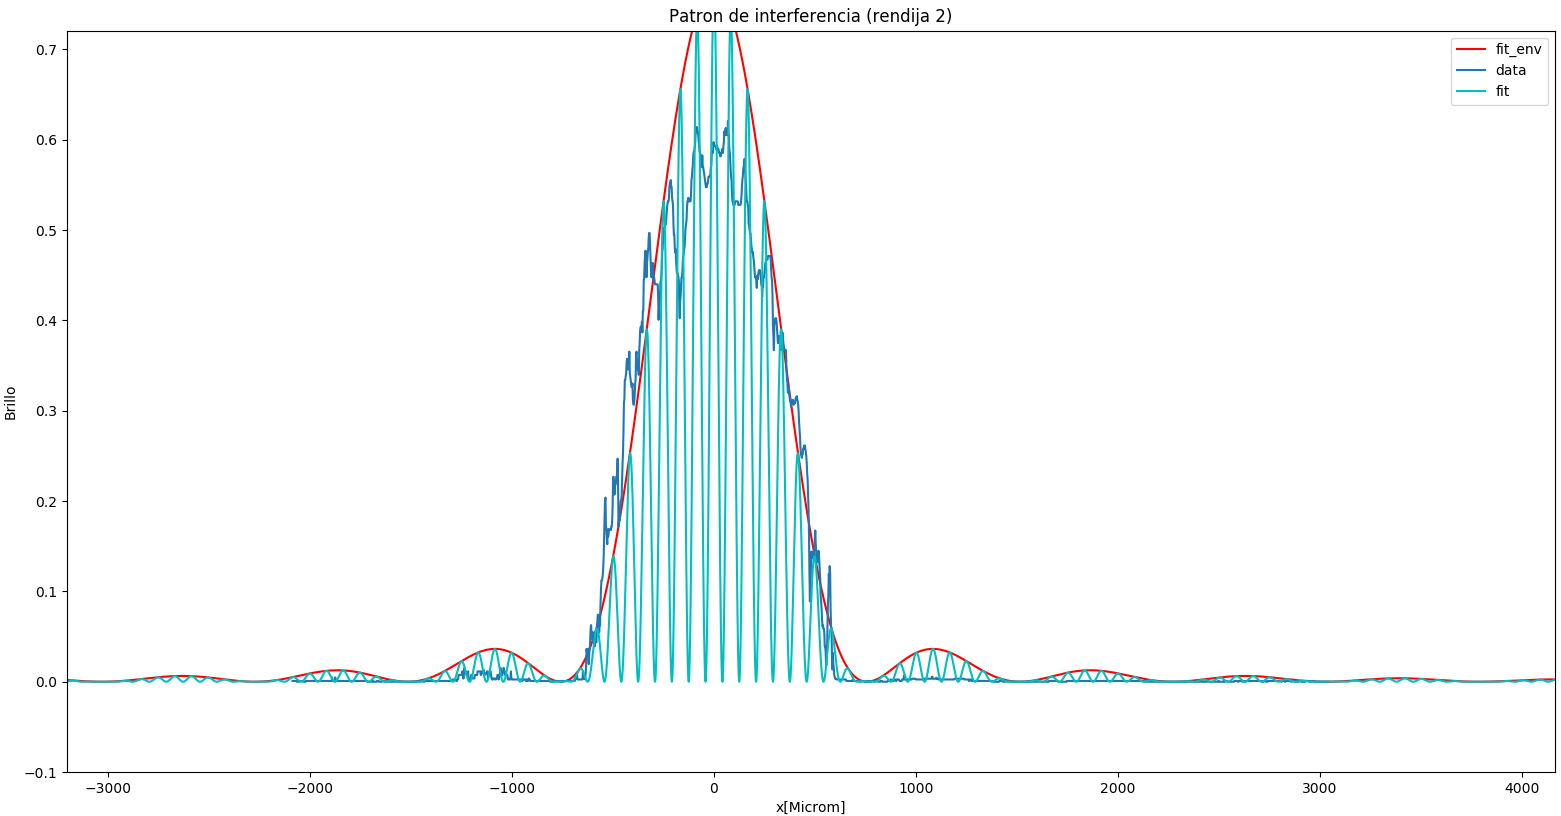
\includegraphics[width=1.0\textwidth]{apg.png}
  \centering
  \caption{Gráfica en del brillo de una hilera de la imagen de doble rendija (Rendija 2, imagen 1)}
\end{figure}

\begin{figure}[h]
  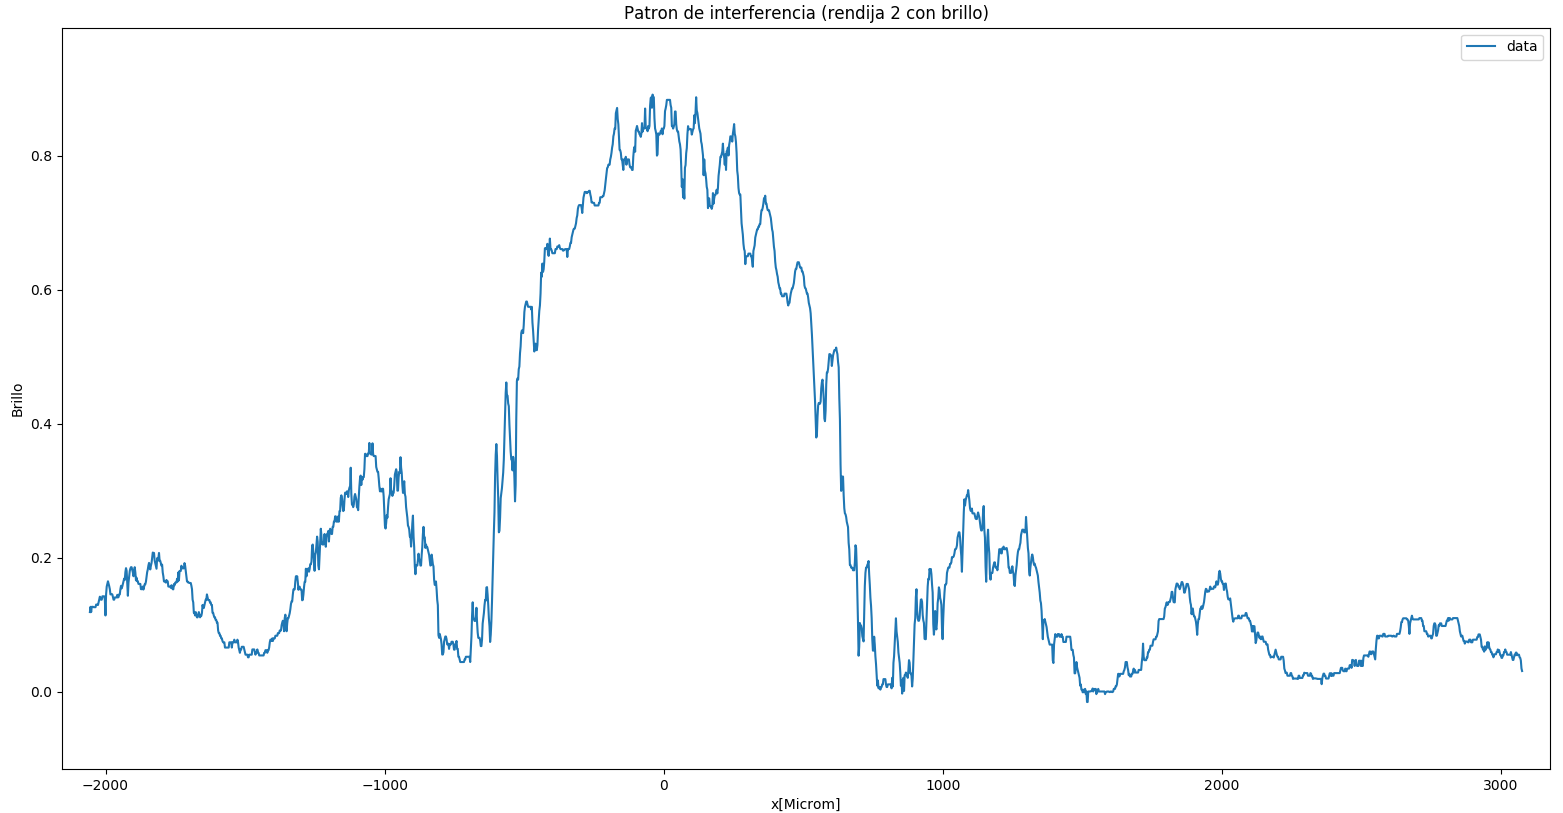
\includegraphics[width=1.0\textwidth]{bpg.png}
  \centering
  \caption{Gráfica en del brillo de una hilera de la imagen de doble rendija (Rendija 2, imagen 2)}
\end{figure} 

\begin{figure}[h]
  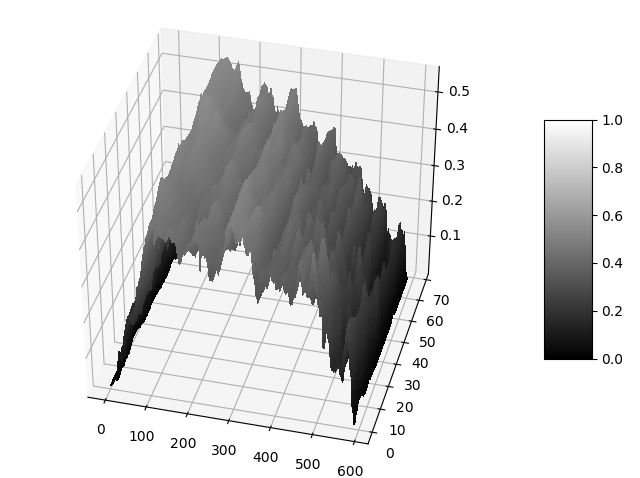
\includegraphics[width=0.6\textwidth]{sp_2D.png}
  \centering
  \caption{Gráfica en 2D del brillo de una franja de la imagen del semiplano}
\end{figure} 

\section{Discucsión}
Considerando que el grosor del cabello humano varía entre $60\mu m$ y $80\mu m$, las mediciones de la primera parte de la práctica resultaron ser valores esperados. El problema es que se usó el mismo cabello para las 3 mediciones, por lo que el grosor no debería de variar más del error de medición entre éstas (algo que, en efecto, ocurre). Ésto se podría derivar de un error de medición, pero estamos bastante seguros de la precisión del experimento. Las variaciones en $\Delta x$ tendrían que ser del orden de 10mm para que las mediciones se parezcan; para z el cambio debería de ser del orden de 10cm (Nótese, por ejemplo, que en el segundo experimento de la rendija simple, aunque el error en z es 40 veces más grande que el de los demás, esto no afecta mucho el error de Wx). Lo que mas seguramente sucedió es que el cabello utilizado tuvo variaciones en su grosor a lo largo de él; las cuales, naturalmente, si pueden ser del orden de la diferencia obtenida.

Para la rendija las mediciones fueron más estables. Ésto probablemente se debió a que fue más facil ajustarla al soporte universal sin que haya variaciones en la altura (a diferencia del cabello, que aunque esté pegado con cinta, cualquier jalón lo resbalaba). No se tenía una medición esperada para el grosor de la rendija, por lo que sólo se puede decir que medimos dicho grosor con una exactitud de alrededor de $5\mu m$.

El análisis de los patrones de interferencia de las dobles rendijas (rendija 1 y rendija 2) fue mas interesante, pero bastante más complicado. Ya se mencionó en la sección de resultados que se tuvieron que realizar algunos retoques de antemano. Ésto no fue suficiente para tener buenos ajustes. Se tuvieron varios otros problemas: Si uno observa a la gráfica de la rendija 1, imagen 2, o a la de rendija 2, imagen 2, puede notar que los mínimos locales en la parte izquierda de la franja principal son notoriamente más grandes (son mas altos) que los mínimos locales de la derecha (lo mismo para máximos locales). Uno puede notar que el origen de éste desajuste (si la impresión de las imágenes es suficientemente buena) es un brillo en la parte izquierda de todas las imágenes (excepto, extrañamente, para la rendija 1, imagen 1 y rendija 2, imagen 1). Este brillo causa incluzo que la "oscuridad" total en la parte izquierda se vea un poco gris; sobre todo si se compara con la parte derecha de las imágenes. Se desconoce exactamente el origen de éste brillo en la parte izquierda (podría ser la luz de la habitación, de las ventanas o lámparas); sólo que ocasiona desajustes terribles. Ésta fue una de las razones por las cuales la primera y la cuarta gráfica no tuvieron ajuste; porque son las que más sufrieron por éste fenómeno. Otro problema importante fue el ajuste del brillo y contraste del detector. El problema se ve claramente al comparar gráficas de imágenes de una misma rendija. Por ejemplo, para la rendija 1, podemos ver que la imagen 2 con brillo más alto tiene una gráfica con intensidad notoriamente más alta que la de rendija 1, imagen 3. Éste comportamiento general es de esperar. El problema es cuando nos fijamos en las proporciones entre el máximo de la franja principal (en imagen 2 es de alrededor de 0.9 y en la imagen 3 es de alrededor de 0.6) y el máximo de las franjas laterales (en la 2 es de 0.4 y en la 3 es de 0.1); las cuales son completamente diferentes.  En los 2 experimentos de la rendija 2, ésto es mucho más notorio; en uno las franjas laterales son casi nulas, y en otro éstas aumentan a una altura de 0.4, cuando la franja principal sólo aumenta en algo menor a 0.3. Esto puede ser causado por la saturación del sensor. Cuando se aumenta la sensibilidad, la franja principal se acerca mucho al tope del rango del instrumento, por lo que mide una intensidad menor a lo que realmente se tiene. Asi que: ¿Cual proporción es la correcta? Con la muestra tan pequeña de imágenes en cada experimento, no estamos seguros; diríamos que ninguna es correcta; si acaso la causa es la que creemos, entonces las de menor sensibilidad. Precisamente éstas fueron a las cuales se realizó el ajuste.

El ajuste al modelo $I(\theta) = A \cos^2 \left ({\frac {\pi d \sin \theta}{\lambda}}\right)~\mathrm{sinc}^2 \left ( \frac {\pi a \sin \theta}{\lambda} \right)$ fue complicado, pues se tenían 3 que ajustar 3 parámetros: $A$ (amplitud máxima), $d$ (distancia entre rendijas) y $a$ (ancho de rendijas). Al intentar ajustar las 3 al mismo tiemo, el programa simplemente se perdía; fijaba 2 y variaba solo una. Una opción era tomar a $A$ como el máximo de la distribución de datos, pero eso sentenciaba a un desajuste total; puesto que al tomar una amplitud así de baja obligaba al programa a tomar una $a$ que formara una franja principal más ancha (que la que se obtuvo al final), lo cual (dado el comportamiento de sinc), recorría drásticamente las franjas laterales hacia un lado. Así, realmente no hubo otra opción mas que hecharle la mano al ajuste y poner con condiciones iniciales a $A$ y $a$ tal que las franjas laterales coincidieran y la gráfica franja principal envolviera a ésta. De ahí, ajustar a $b$ no fue mayor problema.

Para la imágen y gráfica en 2D del semiplano no hay nada mas que decir que se detectó un claro patrón de interferencia cuyo máximo está del lado de la frontera del semiplano y decae con una forma cóncava hacia abajo hacia el punto más alejado de la barrera.

\section{Conclusión}
\noindent Los resultados fueron satisfactorios. Se lograron recrear todos los patrones de interferencia buscados. Se logró medir el diámetro de un cabello con un resultado esperado, pero con diferencias entre mediciones; lo cual puede ser causado por el cambio en el mismo cabello. La medición del grosor de la rendija simple fue más consistente. Lás imágenes de los patrones de interferencia de la doble rendija tuvieron varios problemas. Hay que fijarse que no se tenga una luz como en la de la parte izquierda de muchas imágenes. Pero lo más importante es saber que brillo y contraste tomar. Para esto habría que estar analizando los datos paulatinamente mientras se miden, ajustando el brillo y contraste para que las proporciones de la distribución sean correctas. En el semiplano se observó un patrón de interferencia, mientras que en la imagen no se nota muy peculiar, la gráfica en 2D muestra muy bien su estructura.

\section{Anexo}
Algunas imágenes y gráficas extra.

\begin{figure}[h]
  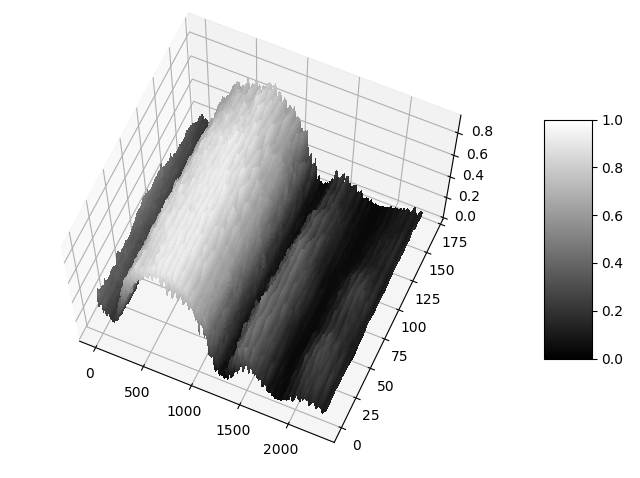
\includegraphics[width=0.6\textwidth]{2_2D.png}
  \centering
  \caption{Gráfica en 2D del brillo de una franja de la imagen de doble rendija (Rendija 1, imagen 2)}
\end{figure} 

\begin{figure}[h]
  
\includegraphics[width=1.0\textwidth]{2p.png}
  \centering
  \caption{Fila de pixeles en doble rendija (Rendija 1, imagen 2)}
\end{figure} 

\begin{figure}[h]
  
\includegraphics[width=1.0\textwidth]{3p.png}
  \centering
  \caption{Fila de pixeles en doble rendija (Rendija 1, imagen 3)}
\end{figure}

\begin{figure}[h]
  
\includegraphics[width=1.0\textwidth]{ap.png}
  \centering
  \caption{Fila de pixeles en doble rendija (Rendija 2, imagen 1)}
\end{figure} 

\begin{figure}[h]
  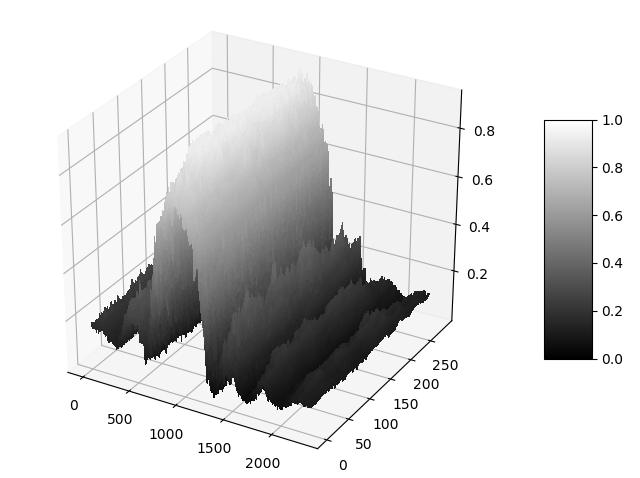
\includegraphics[width=0.6\textwidth]{b_2D.png}
  \centering
  \caption{Gráfica en 2D del brillo de una franja de la imagen de doble rendija (Rendija 2, imagen 2)}
\end{figure} 

\begin{figure}[h]
  
\includegraphics[width=1.0\textwidth]{bp.png}
  \centering
  \caption{Fila de pixeles en doble rendija (Rendija 2, imagen 2)}
\end{figure}

\begin{figure}[h]
  
\includegraphics[width=1.0\textwidth]{spp.png}
  \centering
  \caption{Columna de pixeles en semiplano}
\end{figure} 



\begin{thebibliography}{9}

\bibitem{Física} 
Jackson, J. D. (1975. Berkeley, CA, Estados Unidos de America).
\textit{Classical Electrodynamics}. 
  (2da ed., pp. 269-282). John Wiley \& Sons. Nueva York.


\bibitem{Física} 
Nityananda, R. (2015, Pune, India.)
\textit{Diffraction at a Straight Edge}. 
\\\texttt{https://www.ias.ac.in/article/fulltext/reso/020/05/0389-0400}
Indian Academy of Sciences, Bangalore, India.



\end{thebibliography}
%\begin{thebibliography}{9}
%\bibitem{Física} 
%National Instruments Corporation
%\textit{www.nu.com/es-mx/shop/labview.html}. 
%11500 Mopac Expwy, Austin TX
%\end{thebibliography}
 



\end{document}
%  LocalWords:  KdV
